\setcounter{figure}{0}

\section{2nd July 2023: Memento Mori}
\subsection*{Text: Jonah 1:17-2:1-10}
  \begin{quote}
    [17] And the LORD appointed a great fish to swallow up Jonah. And Jonah was in the belly of the fish three days and three nights

    [1] Then Jonah prayed to the LORD his God from the belly of the fish, [2] saying,

    “I called out to the LORD, out of my distress,
        and he answered me;
    out of the belly of Sheol I cried,
        and you heard my voice.
    [3] For you cast me into the deep,
        into the heart of the seas,
        and the flood surrounded me;
    all your waves and your billows
        passed over me.
    [4] Then I said, ‘I am driven away
        from your sight;
    yet I shall again look
        upon your holy temple.’
    [5] The waters closed in over me to take my life;
        the deep surrounded me;
    weeds were wrapped about my head
    [6]     at the roots of the mountains.
    I went down to the land
        whose bars closed upon me forever;
    yet you brought up my life from the pit,
        O LORD my God.
    [7] When my life was fainting away,
        I remembered the LORD,
    and my prayer came to you,
        into your holy temple.
    [8] Those who pay regard to vain idols
        forsake their hope of steadfast love.
    [9] But I with the voice of thanksgiving
        will sacrifice to you;
    what I have vowed I will pay.
        Salvation belongs to the LORD!”

    [10] And the LORD spoke to the fish, and it vomited Jonah out upon the dry land.
  \end{quote}
\subsection*{Notes}
\begin{itemize}
  \item{All humans will eventually die. Memento Mori is latin for “remember that you must die”. The remembrance of our mortality is a good remedy and therapy for our wayward hearts. Only when we remember that we must die, will we look to Jesus for life.}
  \item{Chapter 2 of Jonah is a little strange; why is the stubborn and rebellious prophet now saying a prayer of thanksgiving? He would have had rather the sailor throw him overboard than to call upon his God. But now Jonah is calling upon his God with a prayer of thanksgiving. Why? Did anything happen between Jonah being thrown overboard and in the fish swallowing him? We can look for clues in his thanksgiving prayer.}
  \item{In Jonah’s thanksgiving prayer, it is clear that Jonah is very familiar with the psalms. In fact, a lot of Jonah’s psalms quotations allude to Jonah descending into Sheol (Hades in greek). In the mind of the Jews, Sheol is a location in the deep of the earth, that everyone must go to when they die, and when people can only go to when they die. So here, Jonah either had a near death experience or he really died. And when Jonah was about to fall from the sea into Sheol, he prayed to escape Sheol, and God heard his prayer. God then sent a fish to swallow Jonah up and then over the span of three days, Jonah went up from Sheol to the sea, i.e he was resuscitated, and then in the belly of the fish he prayed this thanksgiving prayer for God’s delivering him from sheol.}
  \item{Death strikes fear in the hearts of sinful persons. In Jonah 1, the tempest brought the sailors to worship God, and in Jonah 3, Jonah’s proclamation of judgment led the people in Nineveh to repent. For Jonah, at first he was very arrogant, even telling the sailors to throw him into the sea. But when he came face to face with death, his arrogance melted, and he could do nothing except cry to God for help. }
  \item{So when we remember that we will eventually die, it is a scary thought. It should be a scary thought, because we are created for eternity and for life. Death is not in God’s plan for us when He created us. But yet now after Christ conquered death, God uses death to enter the faithful into glory. So these thoughts about death should awaken us from our spiritual lethargy and into faithfulness. Teach us to number our days, as the Psalmist says. This remembrance of death helps points us to what truly matters. }
  \item{Jonah desired to have his own way, and he wanted to flee from God. But his death experience (or near death experience) showed him that the end of going his own way is death, and that only in God is there life.}
  \item{But having said all these about memento mori, while death is used by God to remind us of our frailty and to enter us into glory, it is a bad thing. As the apostle Paul mentioned, death is our enemy. As mentioned before, we were created for eternal life, not death. Death only came into the world because of our rebellion from God and our separation from God. But in God’s wisdom, He uses death for our salvation. God sent His Son to die on the cross for our sins, to destroy death by tasting death and overcoming it by His divinity, and rising from the dead. This is why Jesus says that one sign of his ministry for the Jews would he the sign of Jonah. And now as mentioned above, death is now an entrance into glory for those who are united with Christ; those who die with Christ will be raised with Christ. }
  \item{God’s mercy welcomes all who turn to him. Because of God’s mercy, the rebellious Jonah can find mercy and forgiveness from God. God always hears our prayer and is merciful to us, even when we feel like we are in Sheol. No matter how forsaken we feel, we can just cry out to God, and God will hear us. On the cross, Jesus cried out “my God, my God, why have you forsaken me”. When Jesus says that, it is an expression of His feeling of separation from God (as experienced in his humanity) as He tastes death (in his humanity). That quotation is actually from the start of Psalm 22. And the end of Psalm 22 actually shows God deliverance, which is shown in Jesus’ resurrection. God does not forsake those who call out to Him, and Jonah showed that through his deliverance, as well as our Lord through His resurrection.}
  % \item{\begin{figure}[H]
  %   \centering
  %   % 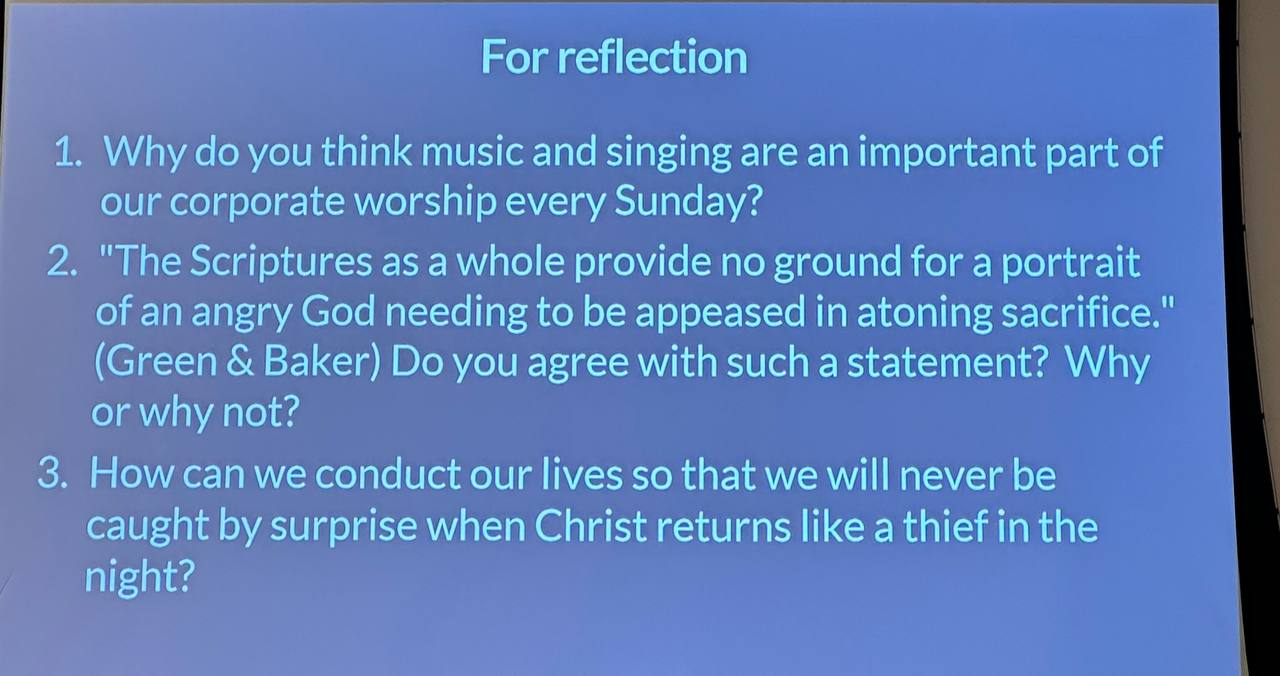
\includegraphics[width=0.8\textwidth, trim={0cm 0cm 0cm 0cm},clip]{Figures/marchSermon4Reflections.jpg}
  %   \includegraphics[width=0.8\textwidth, trim={0cm 0cm 0cm 0cm},clip]{example-image-a}
  %   \caption[]{Reflection questions for this sermon}
  %   \label{}
  % \end{figure}}
\end{itemize}